In this project, we are going to develop a software which will provide the requested behaviours in the Lego Mindstorms EV3 robot. The system overview is shown in figure \ref{fig:robotSystem}, and is briefly described in the following subsections.

\begin{figure}[H]
	\centering
	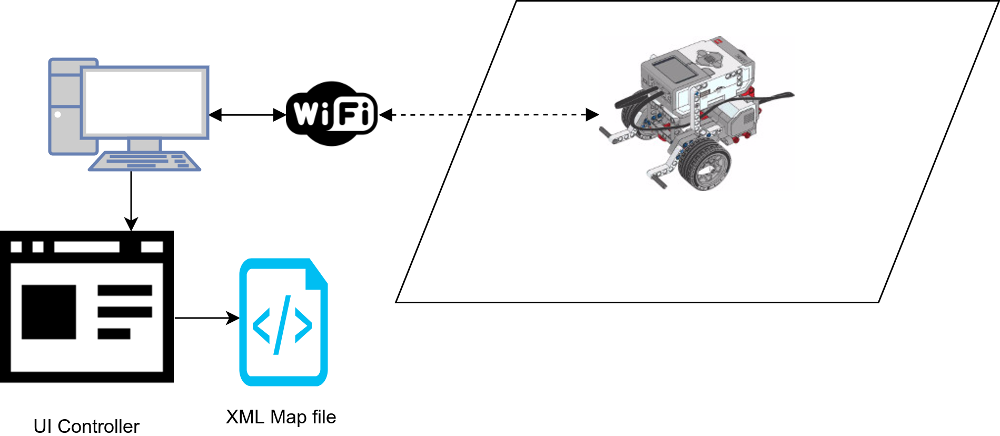
\includegraphics[width=\textwidth]{Robot_system.png}
	\caption{\label{fig:robotSystem} Physical System Overview}
\end{figure}

\subsection{Robot}
A robot will be assembled from the parts provided by the client which should be able to performed all the activities defined in the user requirement section of SRS document. 
\subsection{Computer}
The computer is a platform for several other parts of the system. Including the following sections.

\subsubsection{GUI}
Graphical user interface will be developed to enable the user to interact with system. Buttons and map scene will be provide to control and configure the robot.  
\subsubsection{Manual Controller}
Manual controller is another subsystem of the project which will enable the robot operator to control the robot manually by using the the provided GUI. 
\subsubsection{Auto Controller}
Auto controller will enable the robot to perform some operations like doing survey, avoid obstacles etc. automatically. 
\subsubsection{Map}
The survey map is one of main component of the system. The software will enable the user to load and save the survey map in XML format. The software will also enable the user to zoom on a particular area in the map. 
\subsection{Integration}
Integration will be the key behind the success of this system. Proper integration is required between the above mentioned system components. For connectivity between software and robot, the system will provide different means such as WiFi and bluetooth.  
